\documentclass[]{article}
\usepackage{lmodern}
\usepackage{amssymb,amsmath}
\usepackage{ifxetex,ifluatex}
\usepackage{fixltx2e} % provides \textsubscript
\ifnum 0\ifxetex 1\fi\ifluatex 1\fi=0 % if pdftex
  \usepackage[T1]{fontenc}
  \usepackage[utf8]{inputenc}
\else % if luatex or xelatex
  \ifxetex
    \usepackage{mathspec}
  \else
    \usepackage{fontspec}
  \fi
  \defaultfontfeatures{Ligatures=TeX,Scale=MatchLowercase}
\fi
% use upquote if available, for straight quotes in verbatim environments
\IfFileExists{upquote.sty}{\usepackage{upquote}}{}
% use microtype if available
\IfFileExists{microtype.sty}{%
\usepackage{microtype}
\UseMicrotypeSet[protrusion]{basicmath} % disable protrusion for tt fonts
}{}
\usepackage[margin=1in]{geometry}
\usepackage{hyperref}
\hypersetup{unicode=true,
            pdftitle={Charactersing effect of anaemia on mortality in severe malaria},
            pdfborder={0 0 0},
            breaklinks=true}
\urlstyle{same}  % don't use monospace font for urls
\usepackage{color}
\usepackage{fancyvrb}
\newcommand{\VerbBar}{|}
\newcommand{\VERB}{\Verb[commandchars=\\\{\}]}
\DefineVerbatimEnvironment{Highlighting}{Verbatim}{commandchars=\\\{\}}
% Add ',fontsize=\small' for more characters per line
\usepackage{framed}
\definecolor{shadecolor}{RGB}{248,248,248}
\newenvironment{Shaded}{\begin{snugshade}}{\end{snugshade}}
\newcommand{\KeywordTok}[1]{\textcolor[rgb]{0.13,0.29,0.53}{\textbf{#1}}}
\newcommand{\DataTypeTok}[1]{\textcolor[rgb]{0.13,0.29,0.53}{#1}}
\newcommand{\DecValTok}[1]{\textcolor[rgb]{0.00,0.00,0.81}{#1}}
\newcommand{\BaseNTok}[1]{\textcolor[rgb]{0.00,0.00,0.81}{#1}}
\newcommand{\FloatTok}[1]{\textcolor[rgb]{0.00,0.00,0.81}{#1}}
\newcommand{\ConstantTok}[1]{\textcolor[rgb]{0.00,0.00,0.00}{#1}}
\newcommand{\CharTok}[1]{\textcolor[rgb]{0.31,0.60,0.02}{#1}}
\newcommand{\SpecialCharTok}[1]{\textcolor[rgb]{0.00,0.00,0.00}{#1}}
\newcommand{\StringTok}[1]{\textcolor[rgb]{0.31,0.60,0.02}{#1}}
\newcommand{\VerbatimStringTok}[1]{\textcolor[rgb]{0.31,0.60,0.02}{#1}}
\newcommand{\SpecialStringTok}[1]{\textcolor[rgb]{0.31,0.60,0.02}{#1}}
\newcommand{\ImportTok}[1]{#1}
\newcommand{\CommentTok}[1]{\textcolor[rgb]{0.56,0.35,0.01}{\textit{#1}}}
\newcommand{\DocumentationTok}[1]{\textcolor[rgb]{0.56,0.35,0.01}{\textbf{\textit{#1}}}}
\newcommand{\AnnotationTok}[1]{\textcolor[rgb]{0.56,0.35,0.01}{\textbf{\textit{#1}}}}
\newcommand{\CommentVarTok}[1]{\textcolor[rgb]{0.56,0.35,0.01}{\textbf{\textit{#1}}}}
\newcommand{\OtherTok}[1]{\textcolor[rgb]{0.56,0.35,0.01}{#1}}
\newcommand{\FunctionTok}[1]{\textcolor[rgb]{0.00,0.00,0.00}{#1}}
\newcommand{\VariableTok}[1]{\textcolor[rgb]{0.00,0.00,0.00}{#1}}
\newcommand{\ControlFlowTok}[1]{\textcolor[rgb]{0.13,0.29,0.53}{\textbf{#1}}}
\newcommand{\OperatorTok}[1]{\textcolor[rgb]{0.81,0.36,0.00}{\textbf{#1}}}
\newcommand{\BuiltInTok}[1]{#1}
\newcommand{\ExtensionTok}[1]{#1}
\newcommand{\PreprocessorTok}[1]{\textcolor[rgb]{0.56,0.35,0.01}{\textit{#1}}}
\newcommand{\AttributeTok}[1]{\textcolor[rgb]{0.77,0.63,0.00}{#1}}
\newcommand{\RegionMarkerTok}[1]{#1}
\newcommand{\InformationTok}[1]{\textcolor[rgb]{0.56,0.35,0.01}{\textbf{\textit{#1}}}}
\newcommand{\WarningTok}[1]{\textcolor[rgb]{0.56,0.35,0.01}{\textbf{\textit{#1}}}}
\newcommand{\AlertTok}[1]{\textcolor[rgb]{0.94,0.16,0.16}{#1}}
\newcommand{\ErrorTok}[1]{\textcolor[rgb]{0.64,0.00,0.00}{\textbf{#1}}}
\newcommand{\NormalTok}[1]{#1}
\usepackage{graphicx,grffile}
\makeatletter
\def\maxwidth{\ifdim\Gin@nat@width>\linewidth\linewidth\else\Gin@nat@width\fi}
\def\maxheight{\ifdim\Gin@nat@height>\textheight\textheight\else\Gin@nat@height\fi}
\makeatother
% Scale images if necessary, so that they will not overflow the page
% margins by default, and it is still possible to overwrite the defaults
% using explicit options in \includegraphics[width, height, ...]{}
\setkeys{Gin}{width=\maxwidth,height=\maxheight,keepaspectratio}
\IfFileExists{parskip.sty}{%
\usepackage{parskip}
}{% else
\setlength{\parindent}{0pt}
\setlength{\parskip}{6pt plus 2pt minus 1pt}
}
\setlength{\emergencystretch}{3em}  % prevent overfull lines
\providecommand{\tightlist}{%
  \setlength{\itemsep}{0pt}\setlength{\parskip}{0pt}}
\setcounter{secnumdepth}{0}
% Redefines (sub)paragraphs to behave more like sections
\ifx\paragraph\undefined\else
\let\oldparagraph\paragraph
\renewcommand{\paragraph}[1]{\oldparagraph{#1}\mbox{}}
\fi
\ifx\subparagraph\undefined\else
\let\oldsubparagraph\subparagraph
\renewcommand{\subparagraph}[1]{\oldsubparagraph{#1}\mbox{}}
\fi

%%% Use protect on footnotes to avoid problems with footnotes in titles
\let\rmarkdownfootnote\footnote%
\def\footnote{\protect\rmarkdownfootnote}

%%% Change title format to be more compact
\usepackage{titling}

% Create subtitle command for use in maketitle
\newcommand{\subtitle}[1]{
  \posttitle{
    \begin{center}\large#1\end{center}
    }
}

\setlength{\droptitle}{-2em}
  \title{Charactersing effect of anaemia on mortality in severe malaria}
  \pretitle{\vspace{\droptitle}\centering\huge}
  \posttitle{\par}
  \author{}
  \preauthor{}\postauthor{}
  \date{}
  \predate{}\postdate{}


\begin{document}
\maketitle

{
\setcounter{tocdepth}{2}
\tableofcontents
}
\section{Background}\label{background}

This looks at the severe malaria legacy dataset from MORU

\begin{Shaded}
\begin{Highlighting}[]
\KeywordTok{library}\NormalTok{(lme4)}
\end{Highlighting}
\end{Shaded}

\begin{verbatim}
## Loading required package: Matrix
\end{verbatim}

\begin{Shaded}
\begin{Highlighting}[]
\CommentTok{# For the GAM modelling}
\KeywordTok{library}\NormalTok{(mgcv)}
\end{Highlighting}
\end{Shaded}

\begin{verbatim}
## Loading required package: nlme
\end{verbatim}

\begin{verbatim}
## 
## Attaching package: 'nlme'
\end{verbatim}

\begin{verbatim}
## The following object is masked from 'package:lme4':
## 
##     lmList
\end{verbatim}

\begin{verbatim}
## This is mgcv 1.8-22. For overview type 'help("mgcv-package")'.
\end{verbatim}

\begin{Shaded}
\begin{Highlighting}[]
\CommentTok{# For the CART modelling}
\KeywordTok{library}\NormalTok{(rpart)}
\KeywordTok{library}\NormalTok{(rpart.plot)}
\end{Highlighting}
\end{Shaded}

\section{Exploratory analysis}\label{exploratory-analysis}

Let's look at the key predictive variables. We use a random effects term
to model differences between studies.

\begin{Shaded}
\begin{Highlighting}[]
\KeywordTok{par}\NormalTok{(}\DataTypeTok{las=}\DecValTok{1}\NormalTok{, }\DataTypeTok{mfrow=}\KeywordTok{c}\NormalTok{(}\DecValTok{2}\NormalTok{,}\DecValTok{2}\NormalTok{))}
\NormalTok{## Base Excess and HCT}
\KeywordTok{plot}\NormalTok{(}\KeywordTok{jitter}\NormalTok{(Leg_data}\OperatorTok{$}\NormalTok{HCT,}\DataTypeTok{amount=}\DecValTok{1}\NormalTok{), }\KeywordTok{jitter}\NormalTok{(Leg_data}\OperatorTok{$}\NormalTok{BD), }
     \DataTypeTok{col=}\NormalTok{Leg_data}\OperatorTok{$}\NormalTok{studyID, }\DataTypeTok{pch=}\StringTok{'*'}\NormalTok{, }\DataTypeTok{xlab=}\StringTok{'Haematocrit'}\NormalTok{, }\DataTypeTok{ylab=}\StringTok{'Base Deficit'}\NormalTok{)}
\KeywordTok{legend}\NormalTok{(}\StringTok{'topright'}\NormalTok{, }\DataTypeTok{col=}\KeywordTok{unique}\NormalTok{(Leg_data}\OperatorTok{$}\NormalTok{studyID), }\DataTypeTok{legend =} \KeywordTok{unique}\NormalTok{(Leg_data}\OperatorTok{$}\NormalTok{studyID), }\DataTypeTok{pch=}\StringTok{'*'}\NormalTok{)}
\NormalTok{mod =}\StringTok{ }\KeywordTok{lmer}\NormalTok{(}\DataTypeTok{formula =}\NormalTok{ BD }\OperatorTok{~}\StringTok{ }\NormalTok{HCT }\OperatorTok{+}\StringTok{ }\NormalTok{(}\DecValTok{1} \OperatorTok{|}\StringTok{ }\NormalTok{studyID), }\DataTypeTok{data =}\NormalTok{ Leg_data)}
\NormalTok{ys =}\StringTok{ }\KeywordTok{predict}\NormalTok{(}\DataTypeTok{object =}\NormalTok{ mod, }\DataTypeTok{newdata =} \KeywordTok{data.frame}\NormalTok{(}\DataTypeTok{HCT=}\DecValTok{8}\OperatorTok{:}\DecValTok{50}\NormalTok{, }\DataTypeTok{studyID=}\OtherTok{NA}\NormalTok{), }\DataTypeTok{re.form=}\OtherTok{NA}\NormalTok{)}
\KeywordTok{lines}\NormalTok{(}\DecValTok{8}\OperatorTok{:}\DecValTok{50}\NormalTok{, ys, }\DataTypeTok{lwd=}\DecValTok{3}\NormalTok{, }\DataTypeTok{col=}\StringTok{'black'}\NormalTok{)}

\NormalTok{## Parasitaemia and Anaemia}
\KeywordTok{plot}\NormalTok{(}\KeywordTok{jitter}\NormalTok{(Leg_data}\OperatorTok{$}\NormalTok{HCT,}\DataTypeTok{amount=}\DecValTok{1}\NormalTok{), Leg_data}\OperatorTok{$}\NormalTok{LPAR, }
     \DataTypeTok{col=}\NormalTok{Leg_data}\OperatorTok{$}\NormalTok{studyID, }\DataTypeTok{pch=}\StringTok{'*'}\NormalTok{, }\DataTypeTok{xlab=}\StringTok{'Haematocrit'}\NormalTok{, }\DataTypeTok{ylab=}\StringTok{'Log10 Parasitaemia'}\NormalTok{)}
\CommentTok{#legend('topright', col=unique(Leg_data$studyID), legend = unique(Leg_data$studyID), pch='*')}
\NormalTok{mod =}\StringTok{ }\KeywordTok{lmer}\NormalTok{(}\DataTypeTok{formula =}\NormalTok{ LPAR }\OperatorTok{~}\StringTok{ }\NormalTok{HCT }\OperatorTok{+}\StringTok{ }\NormalTok{(}\DecValTok{1} \OperatorTok{|}\StringTok{ }\NormalTok{studyID), }\DataTypeTok{data =}\NormalTok{ Leg_data)}
\NormalTok{ys =}\StringTok{ }\KeywordTok{predict}\NormalTok{(}\DataTypeTok{object =}\NormalTok{ mod, }\DataTypeTok{newdata =} \KeywordTok{data.frame}\NormalTok{(}\DataTypeTok{HCT=}\DecValTok{8}\OperatorTok{:}\DecValTok{50}\NormalTok{, }\DataTypeTok{studyID=}\OtherTok{NA}\NormalTok{), }\DataTypeTok{re.form=}\OtherTok{NA}\NormalTok{)}
\KeywordTok{lines}\NormalTok{(}\DecValTok{8}\OperatorTok{:}\DecValTok{50}\NormalTok{, ys, }\DataTypeTok{lwd=}\DecValTok{3}\NormalTok{, }\DataTypeTok{col=}\StringTok{'black'}\NormalTok{)}
\NormalTok{## BUN and BD}
\KeywordTok{plot}\NormalTok{(}\KeywordTok{jitter}\NormalTok{(Leg_data}\OperatorTok{$}\NormalTok{BUN,}\DataTypeTok{amount=}\DecValTok{1}\NormalTok{), }\KeywordTok{jitter}\NormalTok{(Leg_data}\OperatorTok{$}\NormalTok{BD), }\DataTypeTok{xlim=}\KeywordTok{c}\NormalTok{(}\DecValTok{0}\NormalTok{,}\DecValTok{140}\NormalTok{),}
     \DataTypeTok{col=}\NormalTok{Leg_data}\OperatorTok{$}\NormalTok{studyID, }\DataTypeTok{pch=}\StringTok{'*'}\NormalTok{, }\DataTypeTok{xlab=}\StringTok{'Blood Urea Nitrogen'}\NormalTok{, }\DataTypeTok{ylab=}\StringTok{'Base Deficit'}\NormalTok{)}
\CommentTok{#legend('topright', col=unique(Leg_data$studyID), legend = unique(Leg_data$studyID), pch='*')}
\NormalTok{mod =}\StringTok{ }\KeywordTok{lmer}\NormalTok{(}\DataTypeTok{formula =}\NormalTok{ BD }\OperatorTok{~}\StringTok{ }\NormalTok{BUN }\OperatorTok{+}\StringTok{ }\NormalTok{(}\DecValTok{1} \OperatorTok{|}\StringTok{ }\NormalTok{studyID), }\DataTypeTok{data =}\NormalTok{ Leg_data)}
\NormalTok{ys =}\StringTok{ }\KeywordTok{predict}\NormalTok{(}\DataTypeTok{object =}\NormalTok{ mod, }\DataTypeTok{newdata =} \KeywordTok{data.frame}\NormalTok{(}\DataTypeTok{BUN=}\DecValTok{5}\OperatorTok{:}\DecValTok{140}\NormalTok{, }\DataTypeTok{studyID=}\OtherTok{NA}\NormalTok{), }\DataTypeTok{re.form=}\OtherTok{NA}\NormalTok{)}
\KeywordTok{lines}\NormalTok{(}\DecValTok{5}\OperatorTok{:}\DecValTok{140}\NormalTok{, ys, }\DataTypeTok{lwd=}\DecValTok{3}\NormalTok{, }\DataTypeTok{col=}\StringTok{'black'}\NormalTok{)}

\NormalTok{## Parasitaemia and Anaemia}
\KeywordTok{plot}\NormalTok{(}\KeywordTok{jitter}\NormalTok{(Leg_data}\OperatorTok{$}\NormalTok{AgeInYear,}\DataTypeTok{amount=}\DecValTok{1}\NormalTok{), Leg_data}\OperatorTok{$}\NormalTok{HCT, }
     \DataTypeTok{col=}\NormalTok{Leg_data}\OperatorTok{$}\NormalTok{studyID, }\DataTypeTok{pch=}\StringTok{'*'}\NormalTok{, }\DataTypeTok{xlab=}\StringTok{'Age in years'}\NormalTok{, }\DataTypeTok{ylab=}\StringTok{'Haematocrit'}\NormalTok{)}
\CommentTok{#legend('topright', col=unique(Leg_data$studyID), legend = unique(Leg_data$studyID), pch='*')}
\NormalTok{mod =}\StringTok{ }\KeywordTok{lmer}\NormalTok{(}\DataTypeTok{formula =}\NormalTok{ HCT }\OperatorTok{~}\StringTok{ }\NormalTok{AgeInYear }\OperatorTok{+}\StringTok{ }\NormalTok{(}\DecValTok{1} \OperatorTok{|}\StringTok{ }\NormalTok{studyID), }\DataTypeTok{data =}\NormalTok{ Leg_data)}
\NormalTok{ys =}\StringTok{ }\KeywordTok{predict}\NormalTok{(}\DataTypeTok{object =}\NormalTok{ mod, }\DataTypeTok{newdata =} \KeywordTok{data.frame}\NormalTok{(}\DataTypeTok{AgeInYear=}\DecValTok{0}\OperatorTok{:}\DecValTok{80}\NormalTok{, }\DataTypeTok{studyID=}\OtherTok{NA}\NormalTok{), }\DataTypeTok{re.form=}\OtherTok{NA}\NormalTok{)}
\KeywordTok{lines}\NormalTok{(}\DecValTok{0}\OperatorTok{:}\DecValTok{80}\NormalTok{, ys, }\DataTypeTok{lwd=}\DecValTok{3}\NormalTok{, }\DataTypeTok{col=}\StringTok{'black'}\NormalTok{)}
\end{Highlighting}
\end{Shaded}

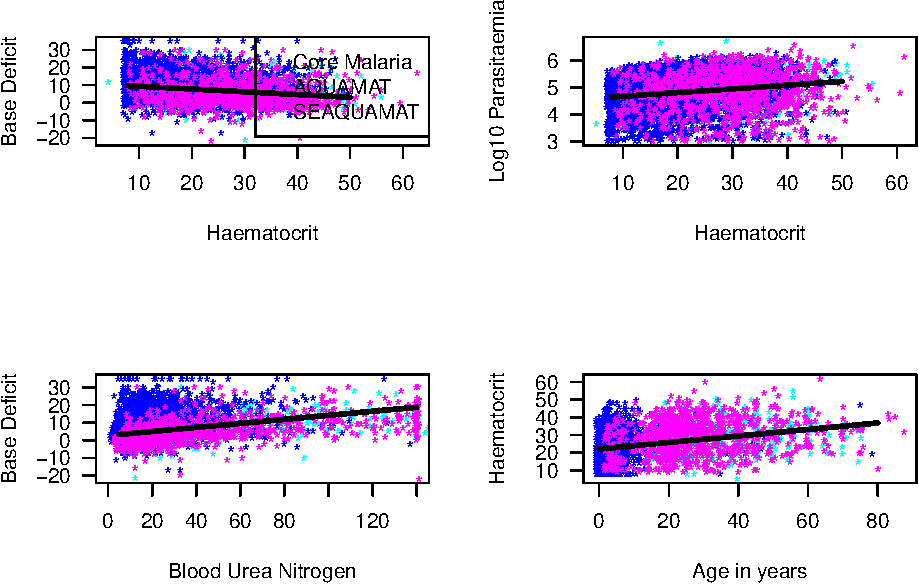
\includegraphics{LegacyAnalysis_files/figure-latex/BD_HCT-1.pdf}

\section{Predictive value of anaemia on death adjusting for
confounders}\label{predictive-value-of-anaemia-on-death-adjusting-for-confounders}

Before fitting the more complex GAM models we explore the standard glm
(logistic regression) models.

\begin{Shaded}
\begin{Highlighting}[]
\NormalTok{mod_full =}\StringTok{ }\KeywordTok{glmer}\NormalTok{(outcome }\OperatorTok{~}\StringTok{ }\NormalTok{HCT }\OperatorTok{+}\StringTok{ }\NormalTok{LPAR }\OperatorTok{+}\StringTok{ }\NormalTok{AgeInYear }\OperatorTok{+}\StringTok{ }\NormalTok{BUN }\OperatorTok{+}\StringTok{ }\NormalTok{BD }\OperatorTok{+}\StringTok{ }\NormalTok{(}\DecValTok{1} \OperatorTok{|}\StringTok{ }\NormalTok{studyID),}
               \DataTypeTok{data=}\NormalTok{Leg_data, }\DataTypeTok{family=}\NormalTok{binomial)}
\end{Highlighting}
\end{Shaded}

\begin{verbatim}
## Warning in checkConv(attr(opt, "derivs"), opt$par, ctrl = control$checkConv, : Model is nearly unidentifiable: very large eigenvalue
##  - Rescale variables?
\end{verbatim}

\begin{Shaded}
\begin{Highlighting}[]
\KeywordTok{summary}\NormalTok{(mod_full)}
\end{Highlighting}
\end{Shaded}

\begin{verbatim}
## Generalized linear mixed model fit by maximum likelihood (Laplace
##   Approximation) [glmerMod]
##  Family: binomial  ( logit )
## Formula: outcome ~ HCT + LPAR + AgeInYear + BUN + BD + (1 | studyID)
##    Data: Leg_data
## 
##      AIC      BIC   logLik deviance df.resid 
##   3214.5   3260.4  -1600.2   3200.5     5221 
## 
## Scaled residuals: 
##     Min      1Q  Median      3Q     Max 
## -3.0755 -0.3426 -0.2344 -0.1681  9.1819 
## 
## Random effects:
##  Groups  Name        Variance Std.Dev.
##  studyID (Intercept) 0.05531  0.2352  
## Number of obs: 5228, groups:  studyID, 3
## 
## Fixed effects:
##              Estimate Std. Error z value Pr(>|z|)    
## (Intercept) -4.216794   0.392658 -10.739  < 2e-16 ***
## HCT          0.019182   0.005440   3.526 0.000422 ***
## LPAR         0.002291   0.066768   0.034 0.972622    
## AgeInYear    0.021372   0.004786   4.465 8.00e-06 ***
## BUN          0.011738   0.001711   6.860 6.87e-12 ***
## BD           0.135063   0.006930  19.491  < 2e-16 ***
## ---
## Signif. codes:  0 '***' 0.001 '**' 0.01 '*' 0.05 '.' 0.1 ' ' 1
## 
## Correlation of Fixed Effects:
##           (Intr) HCT    LPAR   AgInYr BUN   
## HCT       -0.241                            
## LPAR      -0.759 -0.171                     
## AgeInYear -0.269 -0.136  0.030              
## BUN       -0.115  0.074 -0.047 -0.099       
## BD        -0.120  0.254 -0.140  0.070 -0.271
## convergence code: 0
## Model is nearly unidentifiable: very large eigenvalue
##  - Rescale variables?
\end{verbatim}

Now let's make counterfactual predictions of anaemia on death for the
patients in the database:

\begin{Shaded}
\begin{Highlighting}[]
\KeywordTok{par}\NormalTok{(}\DataTypeTok{las=}\DecValTok{1}\NormalTok{)}
\KeywordTok{plot}\NormalTok{(}\OtherTok{NA}\NormalTok{,}\OtherTok{NA}\NormalTok{, }\DataTypeTok{xlim=}\KeywordTok{c}\NormalTok{(}\DecValTok{4}\NormalTok{,}\DecValTok{45}\NormalTok{), }\DataTypeTok{ylim=}\KeywordTok{c}\NormalTok{(}\DecValTok{0}\NormalTok{,}\DecValTok{40}\NormalTok{),}\DataTypeTok{ylab=}\StringTok{'% predicted mortality'}\NormalTok{, }\DataTypeTok{xlab=}\StringTok{'Haematocrit'}\NormalTok{)}
\KeywordTok{title}\NormalTok{(}\StringTok{'Countrerfactual predictions: Overall mortality'}\NormalTok{)}
\ControlFlowTok{for}\NormalTok{(HCT }\ControlFlowTok{in} \DecValTok{4}\OperatorTok{:}\DecValTok{45}\NormalTok{)\{}
\NormalTok{  mydata =}\StringTok{ }\NormalTok{Leg_data}
\NormalTok{  mydata}\OperatorTok{$}\NormalTok{HCT=HCT}
\NormalTok{  ys =}\StringTok{ }\DecValTok{100}\OperatorTok{*}\KeywordTok{predict}\NormalTok{(mod_full, }\DataTypeTok{newdata =}\NormalTok{ mydata, }\DataTypeTok{re.form=}\OtherTok{NA}\NormalTok{, }\DataTypeTok{type=}\StringTok{'response'}\NormalTok{)}
  
  \KeywordTok{points}\NormalTok{(HCT,}\KeywordTok{mean}\NormalTok{(ys), }\DataTypeTok{pch=}\DecValTok{18}\NormalTok{)}
  \KeywordTok{points}\NormalTok{(}\KeywordTok{rep}\NormalTok{(HCT,}\DecValTok{2}\NormalTok{), }\KeywordTok{quantile}\NormalTok{(ys, }\DataTypeTok{probs=}\KeywordTok{c}\NormalTok{(}\FloatTok{0.1}\NormalTok{,}\FloatTok{0.9}\NormalTok{)), }\DataTypeTok{pch=}\StringTok{'-'}\NormalTok{, }\DataTypeTok{col=}\StringTok{'red'}\NormalTok{)}
\NormalTok{\}}
\KeywordTok{abline}\NormalTok{(}\DataTypeTok{h=}\DecValTok{10}\NormalTok{, }\DataTypeTok{lwd=}\DecValTok{3}\NormalTok{, }\DataTypeTok{col=}\StringTok{'blue'}\NormalTok{)}
\end{Highlighting}
\end{Shaded}

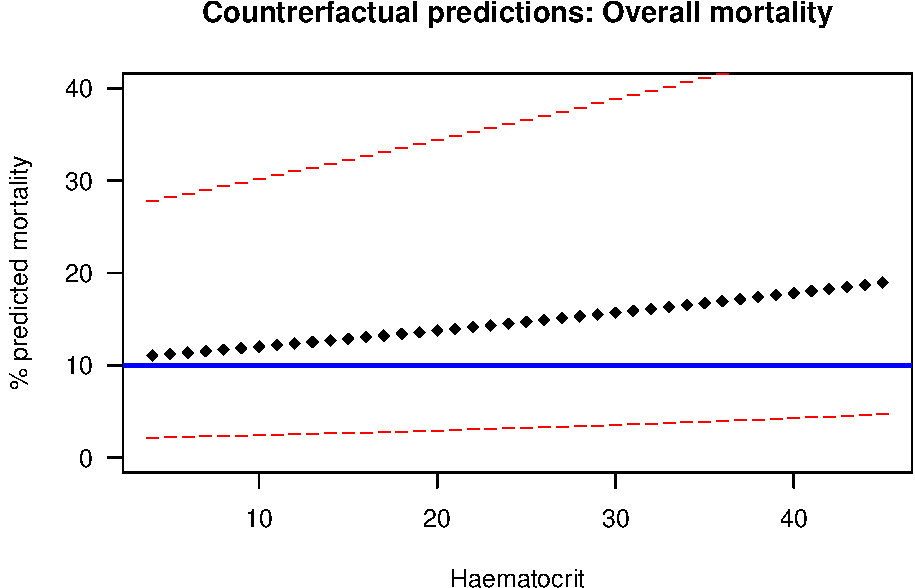
\includegraphics{LegacyAnalysis_files/figure-latex/unnamed-chunk-3-1.pdf}


\end{document}
